\documentclass[12pt]{article}
\usepackage[utf8]{inputenc}
\usepackage{physics}
\usepackage{hyperref}
\usepackage{graphicx}
\hypersetup{
    colorlinks=true,
    linkcolor=blue,
    filecolor=magenta,      
    urlcolor=cyan,
}
\usepackage{amssymb}
\usepackage{ mathrsfs }
\renewcommand{\familydefault}{\sfdefault}

\usepackage{titling}
\renewcommand\maketitlehooka{\null\mbox{}\vfill}
\renewcommand\maketitlehookd{\vfill\null}

\usepackage[a4paper, left=1in, right=1in, top=1in, bottom=1in]{geometry}
\title{\Huge{Notes on Spontaneous Symmetry Breaking}}
\author{\Large{Guru Kalyan Jayasingh}}
\date{\Large{June 2020}}

\begin{document}

\begin{titlingpage}
\maketitle
\end{titlingpage}



\large
\section{Broad Overview of Symmetry Breaking}
Definition:

When the state $\ket{\Psi}$ isn't invariant under the symmetry operator $\hat{U}$
s.t. $\comm{\hat{H}}{U}=0$ (i.e. $\hat{U}$ is a symmetry of the system), then the *\textbf{state}* is said to have spontaneously broken the symmetry.\\
\\
Clarification: Corresponding to every physical symmetry operation (say $\mathcal{G}$, e.g. translation, rotation etc.) of the system, $\exists$ $\hat{U}$ to implement it in $\mathscr{H}$ (the corresponding Hilbert space). \\
$\ket{\Psi}$ violates $\mathcal{G}$, not $\hat{U}$ (what I mean here is that observables that are extracted from $\ket{\Psi}$ don't have the same symmetry as $\mathcal{G}$). \\
\newline
Why is this baffling?\\  
Classically, we reason that since the equations governing the system are symmetric under $\mathcal{G}$, so should the actual state be (here I refer to classical state in a dynamical sense i.e look at macrostates). Hence Spontaneous symmetry breaking (a.k.a SSB) can be thought about understanding how symmetry in microscopic descriptions are broken on a macroscopic/grand scale.\\
Q. Mechanically, one can motivate the idea through the following quandary:-\\
\\
\textbf{Proof that crystals can't exist at all temperatures:}\\
Take the following crytal hamiltonian
$$\hat{H}\;=\;\sum_i \frac{p_i^2}{2m}+\sum_{i<j}V(\Vec{r}_i-\Vec{r_j})$$
Now, arbitrary global translations are a symmetry of $\mathcal{H}$, characterised by the operator $\hat{U}\;=\;\hat{T}_{\Vec{\eta}}$, for $\Vec{\eta}$ being the translation. Also $\comm{\hat{H}}{\hat{T}_{\Vec{\eta}}}=\;0$. Now, in a crystal the density is modulated i.e. $\rho_{obs}(x)\;=\;\rho_{obs}(x+a)$ for $a$ being a crystal translation vector.\\
However look at the following
\begin{align*}
    <\hat{\rho(x+\eta)}> &= \;\frac{1}{Z}Tr(e^{-\beta \hat{H}}\hat{T}_{\Vec{\eta}}\;\hat{\rho}(x)\;\hat{T}^{-1}_{\Vec{\eta}} ) \\
    \implies\; <\hat{\rho(x+\eta)}>\;&=\; <\hat{\rho(x)}>
\end{align*}
Hence density cannot stay modulated and a crystal cannot be observed, contrary to empirical observation. So what gives?\\
Clearly one of our assumptions while using statistical averages is wrong and as it turns out, it's the assumption of \textbf{ergodicity}. We'll see how it comes, but the gist is that on experimental timescales, system cannot explore all parts of the phase space with some statistical weight.\\
\\
Caution: SSB isn't a purely quantum phenomenon.\\
\newline
In the spirit of QFT, one can say that SSB describes systems in which $\mathcal{L}$ has a symmetry, but the lowest order vacuum solutions don't possess the said symmetry (although we'll explore the statistical side of SSB, leaving such cases aside).\\
\\
Observation 1: For every such $\ket{\Psi}$, there exists a multitude of states $\ket{\Phi}$ s.t. they're degenerate. 
One can generate the set {$\ket{\Phi}$} by the rule $\ket{\Phi}\;=\;\hat{U}\ket{\Psi}$.\\
Check that $E_{\ket{\Psi}}\;=\;E_{\ket{\Phi}}\;\;\;\;\;\;\;\;\;\;\;\;\;\;\;\;\;\;\;\;\;\;\;\;\;\;\;\;\;\;\;\;\;\;\;\;\;\;\;\;\;\;\;\;\;\;\;\;\;\;\;\;\;\;\;\;\;\;\;\;\;\;\;--(1)$.\\ 
\newline
Order Parameter Operator: For the set of *broken* symmetry states, one can define an order parameter operator $\hat{O}$.
The action of this operator is defined as:
\begin{itemize}
    \item 
        Each of the symmetry related states {$\ket{\Phi}$} are the eigenstates of this operator with distinct non-zero eigenvalues.
    \item The expectation value $\hat{O}$ in a symmetric state is 0. 
\end{itemize}
In general $\comm{\hat{O}}{\hat{H}}\neq 0$ (however $\exists$ exceptional *cases* where it happens to be true).\\
\\
Observation 2: For the general case, we can see that $\ket{\Psi}$ will not be an Energy eigenstate. Moreover, it cannot be a thermal mixture of energy eigenstates.\\
Proof: Taking $\comm{\hat{O}}{\hat{H}}\neq 0$, it can't be an eigenket since that would imply $\hat{H}$ and $\hat{O}$ commute.
For the thermal mixture case (?) - e.g. Crystal fallacy above.\\
\newline
Conclusion: Clearly the symmetry broken state $\ket{\Psi}$ isn't in a thermal equilibrium! Then shouldn't these states be unstable? 
No. We do get to observe them in day-day life and these clearly unequivocally exist with large lifetimes(and hence are stable in the colloquial sense).
How does this happen then? Ans - Due to the large singularity of thermodynamic limit. \\
At Thermodynamic limit( $N\rightarrow \infty$, $V\rightarrow \infty$ with $\displaystyle{\frac{N}{V}=\; constant}$) :
\begin{itemize}
    \item  $<\comm{\hat{H}}{\hat{O}}>\;=\;0$
    \item SSB states become orthogonal to each other i.e. $\braket{\Phi}{\Psi}=0$
    \item SSB states become degenerate with Symmetric energy eigenstates, thus becoming eigenstates themselves. Hence they can occur in thermal equilibrium.
\end{itemize}
These states can therefore \textbf{exist} in the thermodynamic limit.\\
Thermodynamic limit, being qualitatively different as above from large finite N,V makes the limit itself a singular one(defined below). Ergo - Thermodynamic limit is an idealisation, only to serve as a guide and not a real description.
\subsection{What happens for finite N?}
Observation 3: Symmetric Hamiltonians (by symmetry here a global symmetry is implied) exhibit the following properties:

\begin{itemize}
    \item The decompostion of $\hat{H}\;=\;\hat{H_0} + \sum_{\Vec{K}}\hat{H}_{\Vec{K}}$ is possible, where the 1st part realizes $\Vec{k}=0$ part of the F.T. i.e. Centre of Mass part and the 2nd part describes internal degrees of freedom(basically a fourier decomposition into different non-zero and zero $\Vec{k}$ parts).
    \item $\comm{\hat{H}_0}{\sum_{\Vec{K}}\hat{H}_{\Vec{K}}}\;=\;0$
\end{itemize}\\
\textbf{Question}: What if the quantity $H_0\;=\int \hat{H}(\Vec{r_i},\Vec{p_i})\; \Pi_{i=1}^N d^3\Vec{r_i}$ diverges?\\ Since energy is an extensive property of the system, won't it exclusively depend on the volume of the system as such (for e.g. set $\hat{H_0}\;=\;\hat{H}_{SHO})$?\\
\\
Claim: The \textbf{global} symmetry breaking can be explained only by using $\hat{H}_0$ part of $\hat{H}$.\\
\\
Example: For a solid, the exact hamiltonian looks like 
$$\hat{H}\;=\;\sum_i \frac{p_i^2}{2m}+\sum_{i<j}V(\Vec{r}_i-\Vec{r_j})$$
Although the system has translational symmetry, when we observe daily life objects like a rock, they don't exhibit the symmetry of the hamiltonian i.e. they aren't delocalised over all space. Now for this, the collective part of the hamiltonian describes the C.O.M motion or the motion of N atoms on mass m moving in unison.\\
In free space, this motion corresponds to a free particle with M = mN and the lowest energy level spacing scales as $\frac{1}{N}$.\\


\textbf{Tower of States}: 
These low lying energy levels of the solid makeup what's called the \textbf{tower of states}.
Important to note that the states( which are eigenstates of $\hat{\Vec{P}}_{total}$ and hence behave like a \textbf{delocalised wave} over the whole space) are collective excitations of the whole system and as such are non-local.\\
\\
Non local in what sense? - Can't be written as $\bigotimes \ket{\Psi}_j$, for $\ket{\Psi}_j$ being single particle states(in a general basis that is).
Because they're non-local, as the system size increases, they become increasingly unstable towards local interactions, hence not observed in daily life(\textbf{Why?}).\\
\\
\textbf{Question}: Why is the GS of the true system only the eigenstate of the collective part?\\
(It seems plausible on energy grounds, since the collective part shall offer lowest energy, but the argument is motivated by a classical picture - basically net energy of the system = $E_{COM}$ + $E_{system\;wrt\;COM}$, hence lowest energy contributions come from COM)\\
\\
Now what happens to stable states in this analysis?
\begin{itemize}
    \item Clearly they aren't one of these low lying\textbf{ symmetric}( i.e. wrt global symmetry of the system, for e.g. in case of a solid, states exhibiting translational invariance) eigenstates of the collective hamiltonian.\\
    This is from daily observation that these states are the normal SSB states.
    \item If not eigenstates, then these are superpositions of the low lying eigenstates (\textbf{Why?}).
    \item Now since low lying energy gap scales as $\displaystyle{\frac{1}{N}}$, for large N, they squeeze up and hence the energy uncertainty reduces for the stable SSB state.
    \item This makes them almost degenerate(i.e. $<E> \approx E_n$) in the large N limit and has energy close to exact GS of the hamiltonian(\textbf{Why?}).
    \item Overlap between SSB states now scales as $\exp{-N}$ and hence tunneling probability to another SSB state is suppressed.
    
    
    \item Why are they stable? Simply because they are local(unlike the symmetric states), can be written as  $\bigotimes \ket{\Psi}_j$ and are stable against local perturbations. 
   
\end{itemize}
\\
Now for finite N, a symmetric H clearly cannot induce an SSB GS. One is forced to consider a \textbf{symmetry breaking perturbation} that singles out a particular SSB state out of the many degenerate,stable SSB states.\\
Why the Spontaneous(the 1st \text{S}) in SSB? - Large system are exceedingly sensitive to even a small perturbation. Latter  suffices to single out a particular SSB state. Hence the termed "Spontaneus".\\
\\
$\hat{H}_0\;+\;\hat{H}_{sb\;perturb}$ = SSB GS of the full system!\\
In thermodynamic limit, the GS is an eigenstate of the order parameter operator (why? - Since here SSB states are orthogonal).\\
But without $\hat{H}_{sb\;perturb}$, the GS is symmetric for \textbf{any} system size. This clarifies that the thermodynamic limit is singular - adding or subtracting $\hat{H}_{sb\;perturb}$ changes the fate of GS itself, even qualitatively.\\
\newline
\textbf{The Ergodicity Breakdown}
\begin{itemize}
    \item $\braket{\Phi_{ssb}}{\Psi_{ssb}}\approx\;\exp(-N)$ - exponentially suppressed.
    \item Hence for all practical purposes, one can treat as if the system has only \textbf{1} SSB GS.
    \item All other SSB states are inaccessible with the entire dynamics taking place in the particular SSB state and it's excitations.
    \item Ergodicity breaks - System only lives( "explores") a restricted Hilbert space. The rest of phase space isn't accessible on \textbf{experimental timescales}.
    \item However, if one wants to study physics of phase transitions, then clearly the system visits a different SSB GS.
    \item Moral - Global Thermal equilibrium isn't reached. Ex: Disordered Glasses
\end{itemize}
Suggested Paper: R. G. Palmer,\textit{ Broken ergodicity}, Adv. Phys. 31, 669 (1982).\\
\href{https://www.tandfonline.com/doi/abs/10.1080/00018738200101438}{doi:10.1080/00018738200101438.}

\section{Singular Limits}
Example of Singular Limit:
$<section\; 2.3 \;and\; 2.4\;>$


\section{A Classical Example: Magnetism}
The idea that different symmetry broken states could be degenerate seems to be at a *conundrum*. For $\ket{\Psi}$, (1) states that SSB states are degenerate (one checks that in (1), $\ket{\phi}$ is a different SSB state since it should in general have different eigenvalue via $\hat{O}$).\\
To explore the same statement in classical physics, one takes following model of a classical magnet
\begin{align}
    \mathcal{H}\;=\;\sum_{\Vec{x},\Vec{\delta}} - \abs{J} \Vec{S}_{\Vec{x}}\cdot\Vec{S}_{\Vec{x }+\Vec{\delta}}
\end{align}
accounting for nearest neighbour interaction.
\begin{enumerate}
    \item For minm. E, align every magnet in same direction.$\exists$ a global $SO(3)$ symmetry of spin rotations in $R^3$, leaving the configurations degenerate.
    \item $<M>$ = $\displaystyle{\frac{e^{(-\beta E_{state})}\cdot M_{state}}{Z}}$ = 0 (think why). So no net magnetisation( at \textbf{any T}).
    \item Above is in a contradiction to the fact that we can see a *net* magnetism at room temp for various substances.
\end{enumerate}
Resolution: Introduce a small symmetry breaking term in $\mathcal{H}$.
\begin{align}
    \mathcal{H}\;=\;\sum_{\Vec{x},\Vec{\delta}} - \abs{J} \Vec{S}_{\Vec{x}}\cdot\Vec{S}_{\Vec{x }+\Vec{\delta}} - h\hat{n}\cdot\Vec{S}_{\Vec{x}}
\end{align}
i.e. essentially add a small magnetic field(set h=0 at the end).\\
Now 
\begin{enumerate}
    \item  $<M>$ = $Ns\hat{n}$ at T=0, for $s= M_{per\;spin}$.( think why)
    \item  A set of non-commuting limits emerge
        \begin{align*}
              &\lim_{h\to 0}\lim_{N\to \infty} \frac{<M>}{N}\;=\;s\\
              &\lim_{N\to \infty}\lim_{h\to 0} \frac{<M>}{N}\;=\;0
        \end{align*}
    \item What do the limits mean for magnets in our everyday world? \\
    Suppose we start with a finite sample of spins and then take the thermodynamic limit of $\lim{N\to\infty}$. Now this limit can be taken at the behest of an **arbitrarily** small magnetic field. First we set $B=0$. Clearly none in the compact sample of spins get magnetised and now if we take thermodynamic limit, we find that the average spin was and still is 0.
    \item Now suppose we ramp up a small $B$ and let the compact sample acquire a small moment. Take $\lim{N\to\infty}$. Switch $B=0$. What we find now is that the sample still has a **net** moment. This holds for arbitrarily weak $B$. The spontaneity of the evolution comes from a qualitative change of outcome even in the presence of a minuscule \textbf{magnetic history}.
\end{enumerate}
Q. What was the point of getting to know "classically SSB states might not be degenerate"? - Clear to see.
Arbitrary
$\hat{n}$ leads to same energy in
$\lim_{h\to 0}$, situation at 0 K.

\section{Harmonic Crystal}
For an explicit example, take the harmonic crystal:-
\begin{equation*}
    \hat{H}\;=\;\sum_{\Vec{x}} \frac{\hat{P}^2(\vec{x})}{2m}+\sum_{\vec{x},\vec{\delta}}\frac{1}{2m}\;(\hat{X}(\vec{x})-\hat{X}(\vec{x}+\vec{\delta})\;)^2
\end{equation*}
where $\delta=\;(a,a,a)$ for a being the crystal spacing.
We calculate here the collective $\mathcal{H}$.\\
\newline
Guess: $\mathcal{H}_{0}\;=\;\mathcal{H}_{COM}$. The COM is a particle of mass mN and momenta $\hat{P}_{COM}\;=\;\sum_i \hat{P}_i$.\\

Observation: $\comm{H}{P_{com}}\;=\;0$.\\

Legal consequences:
\begin{itemize}
    \item All eigenstates of the crystal are total-momentum eigenstates.
    \item $\Delta P_{com}\;=\;0$, then $\Delta X_{com}=?$
    \item So is the GS (i.e. your chair/crystal etc.) is an eigenstate?
    \item Is it a thermal state? ;)
\end{itemize}
\newpage
\subsection{Calculation of the collective Hamiltonian}
$$  \hat{H}_{crystal}\;=\;\hat{H_0} + \sum_{\Vec{K}}\hat{H}_{\Vec{K}}$$
Q. What does $\hat{H}_{\Vec{K}}$ physically indicates?\\
Define formally the fourier transform of the operators as 
\begin{align}
    \hat{X}(\Vec{r})\;&=\;\sum_{\Vec{k}} \hat{X}(\Vec{k}) e^{-i\Vec{k}\cdot\Vec{r}}\\
    \hat{X}(\Vec{k})\;&=\;\int_{\mathcal{V}} e^{+i\Vec{k}\cdot\Vec{r}}\;\hat{X}(\Vec{r})\\
    \hat{X}^{\dagger}(\Vec{k})\;&=\; \hat{X}(-\Vec{k})
\end{align}
In the same vein, we define 
\begin{align}
 \hat{P}(\Vec{r})\;&=\;\sum_{\Vec{k}} \hat{P}(\Vec{k}) e^{i\Vec{k}\cdot\Vec{r}}\\
    \hat{P}(\Vec{k})\;&=\;\int_{\mathcal{V}} e^{-i\Vec{k}\cdot\Vec{r}}\;\hat{P}(\Vec{r})\\
    \hat{P}^{\dagger}(\Vec{k})\;&=\; \hat{P}(-\Vec{k})
\end{align}
The above definition ensures that the commutation relations in the new set are 
\begin{equation}
    \comm{\hat{X}(\Vec{q})}{\hat{P}(\Vec{k})}\;=\;ih\;\delta^3(\Vec{q}-\Vec{k})
\end{equation}
Now,
\begin{align}
    \hat{P}_{com}\;&=\;\sum_{\Vec{x}} \hat{P}(\Vec{x})\\
    \implies \hat{P}_{com}\;&=\sum_{\Vec{x}}\sum_{\Vec{k}} \hat{P}(\Vec{k}) e^{i\Vec{k}\cdot\Vec{x}}\\
    \implies \hat{P}_{com}\;&=\sum_{\Vec{k}} \hat{P}(\Vec{k}) \delta^{3}(\Vec{k})\;\mathcal{V}\\
    \implies \hat{P}_{com}\;&=\;\hat{P}(0)\mathcal{V}
\end{align}
where we used $\sum_{\Vec{r}}e^{i\Vec{k}\cdot\Vec{r}}\;=\;\delta^3(k)\;\mathcal{V}$, with $\mathcal{V}$ being the finite volume of the sample.\\
Also, 
\begin{align}
    \sum_{\Vec{x}} \hat{P}^2(x)\;&=\;\sum_{\Vec{x}}\;\sum_{\Vec{k},\Vec{q}} \hat{P}(\Vec{k})\hat{P}(\Vec{q})\;e^{i(\Vec{k}+\Vec{q})\cdot \Vec{x}}\\
    &=\;\sum_{\Vec{k},\Vec{q}}\hat{P}(\Vec{k})\hat{P}(\Vec{q}) \delta^3(k+q)\;\mathcal{V}\\
    &= \sum_{\Vec{k}} \hat{P}(\Vec{k}) \hat{P}(\Vec{-k}) \;\mathcal{V}
\end{align}
Taking the zero $\Vec{k}$ part, we have 
\begin{align}
     \sum_{\Vec{x}} \hat{P}^2(x)\;&= \hat{P}(\Vec{0}) \hat{P}(\Vec{0})\;\mathcal{V}\\
     &= \frac{1}{\mathcal{V}}\;\hat{P}^2_{com}
\end{align}
Now we can clearly see that( for the $\vec{k}\;=0$ part)
\begin{equation}
    \sum_{\Vec{x}} \frac{1}{2m}\hat{P}^2(x)\;=\;\frac{1}{2m\mathcal{V}}\;\hat{P}^2_{com}\;=\;\frac{\hat{P}^2_{com}}{2mN}
\end{equation}


Since $\mathcal{V} \sim N$. Now we perform the same steps on the harmonic part:-
\begin{equation}
    \sum_{\vec{x},\vec{\delta}} (\hat{X}(\vec{x})-\hat{X}(\vec{x}+\vec{\delta})\;)^2 = 4 \sum_{\vec{k}, \vec{\delta}} \hat{X}(\vec{k})\hat{X}(\vec{-k})\; sin^2(\frac{1}{2}\;\vec{k}\cdot\vec{\delta}) 
\end{equation}
 which yields no part when we take $\vec{k}=0$ part.
 
Hence, to calculate the collective hamiltonian, we take $\vec{k}\;=0$ parts from (17) and (21) to get 
\begin{align}
    \mathcal{H}_{collective}\;&=\;\frac{\hat{P}^2_{com}}{2mN}
\end{align}


\textbf{To explore SSB, we only take $\mathcal{H}_0$ part of $\hat{H}_{crystal}$}.\\
\newline
Why is it valid?
\begin{itemize}
    \item $\comm{P_{com}}{\hat{H}}=0$, hence good quantum numbers \textbf{of} one part are good quantum no.'s of other.
    \item At extremely low temperatures, only the collective part of the Hamiltonian matters.\\
        This is because phonon energies are much-much higher than the spectra of the collective hamiltonian. \textbf{(finite T?)}
\end{itemize}
\newpage
\subsection{$\mathcal{\hat{H}}_0$ Spectrum}
 
\begin{figure}[h]
    \centering
    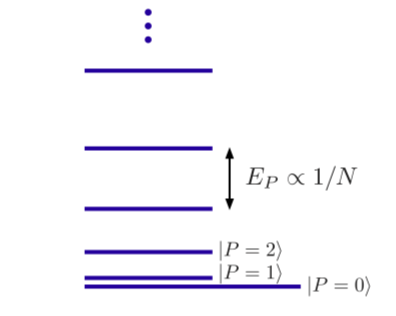
\includegraphics[scale=0.8]{Screen Shot 2020-07-22 at 19.42.20.png}
    \caption{Collective Spectrum}
    \label{fig:my_label}
\end{figure}
\begin{align}
    \mathcal{H}_{collective}\;&=\;\frac{\hat{P}^2_{com}}{2mN}
\end{align}
\begin{enumerate}
    \item G.S: E=0, $\psi\;=1$ everywhere - delocalised with equal phase.
    \item 
    $\Delta E\;\sim\;\frac{1}{N}$, the separation from GS and excitations with non-zero $P_{com}$.
    \item As ${N\to\infty}$, tower collapses. Excited states become degenerate with GS.\\
    No energy needed to excite a collective mode!
    \item To make a crystal, simply make a wavepacket from these states with well defined $X_{com}$. What's $<E_{wavepacket}>$?\\
    Clearly, as ${N\to\infty}$, it's 0. Hence we can see a crystal in thermodynamic limit.
\end{enumerate}
Of course real crystals are \textbf{not infinitely large}, and superpositions of momentum states \textbf{do} cost energy to create.\\
\newline
"How much energy is required for finite N to localise the system?"\\
\newpage
To account for the localisation energy, we add a \textbf{confining} potential that prevents delocalisation - In the end we'll set it to 0.\\
Hence, we go with
\begin{equation}
    H_{pert}\;=\;\frac{\hat{P}^2_{com}}{2mN}+\;\mu X^2_{com}
\end{equation}
where $\mu$ is the strength of a potential that tends to localise the crystal at the origin of our coordinate system. \\
\newline
We get for the perturbed system
\begin{align}
    E_n\;&=\;h\omega\;(n+\frac{1}{2})\\
    \Psi_0(x)\;&=\;(\frac{2mN\mu}{\pi^2h^2})^{\frac{3}{8}}\;e^{\displaystyle{-\sqrt{\frac{mN\mu}{2h^2}}x^2}}
\end{align}
with $\omega\;=\;\sqrt{\displaystyle{\frac{2\mu}{mN}}}$, $\sigma^2\;=\;\displaystyle{\frac{h}{\sqrt{2mN\mu}}}$.\\
Signal of SSB:-
\begin{figure}[h]
    \centering
    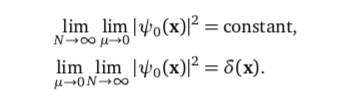
\includegraphics[scale=0.7]{Screen Shot 2020-07-22 at 21.55.01.png}
\end{figure}
\\
2nd limit signifies the \textbf{spontaneous} nature of the limit - for an $\infty$ large system, any perturbation, no matter how weak, is enough to completely localise the wave function in a single position.\\
\newline
Still, what about finite N? - For larger and larger pieces of matter,\\
weaker and weaker perturbation suffices to make its ground state a localised wave packet!\\
\newline
As per an estimate, even with the lowest measurable force ($10^{-21}N, zeptonewton)$, for a 1cc piece of iron, localisation can be done to about $10^{-12}$ m.(2 orders of magnitude smaller than atomic lengthscales).\\
\newline
So we can see that for finite N, the minimum size of perturbation keeps reducing with increasing N.


\newpage
\subsection{Is it thermal ?}
There is some competition between perturbation and thermal fluctuations.\\
Perturbations localise the system(i.e. break symmetry), while thermal fluctuations thermalize the system.\\
So one could in principle replace the formula 
\begin{equation*}
    <G>\;=\;Tr(\rho \;\hat{G})
\end{equation*}
and carry out the trace in the new basis of SSB states, since these are the only stable states. Turns out, this is not correct! (why?)\\
\newline
Why don't we jump from one SSB state to another?\\

\begin{figure}[h]
\centering
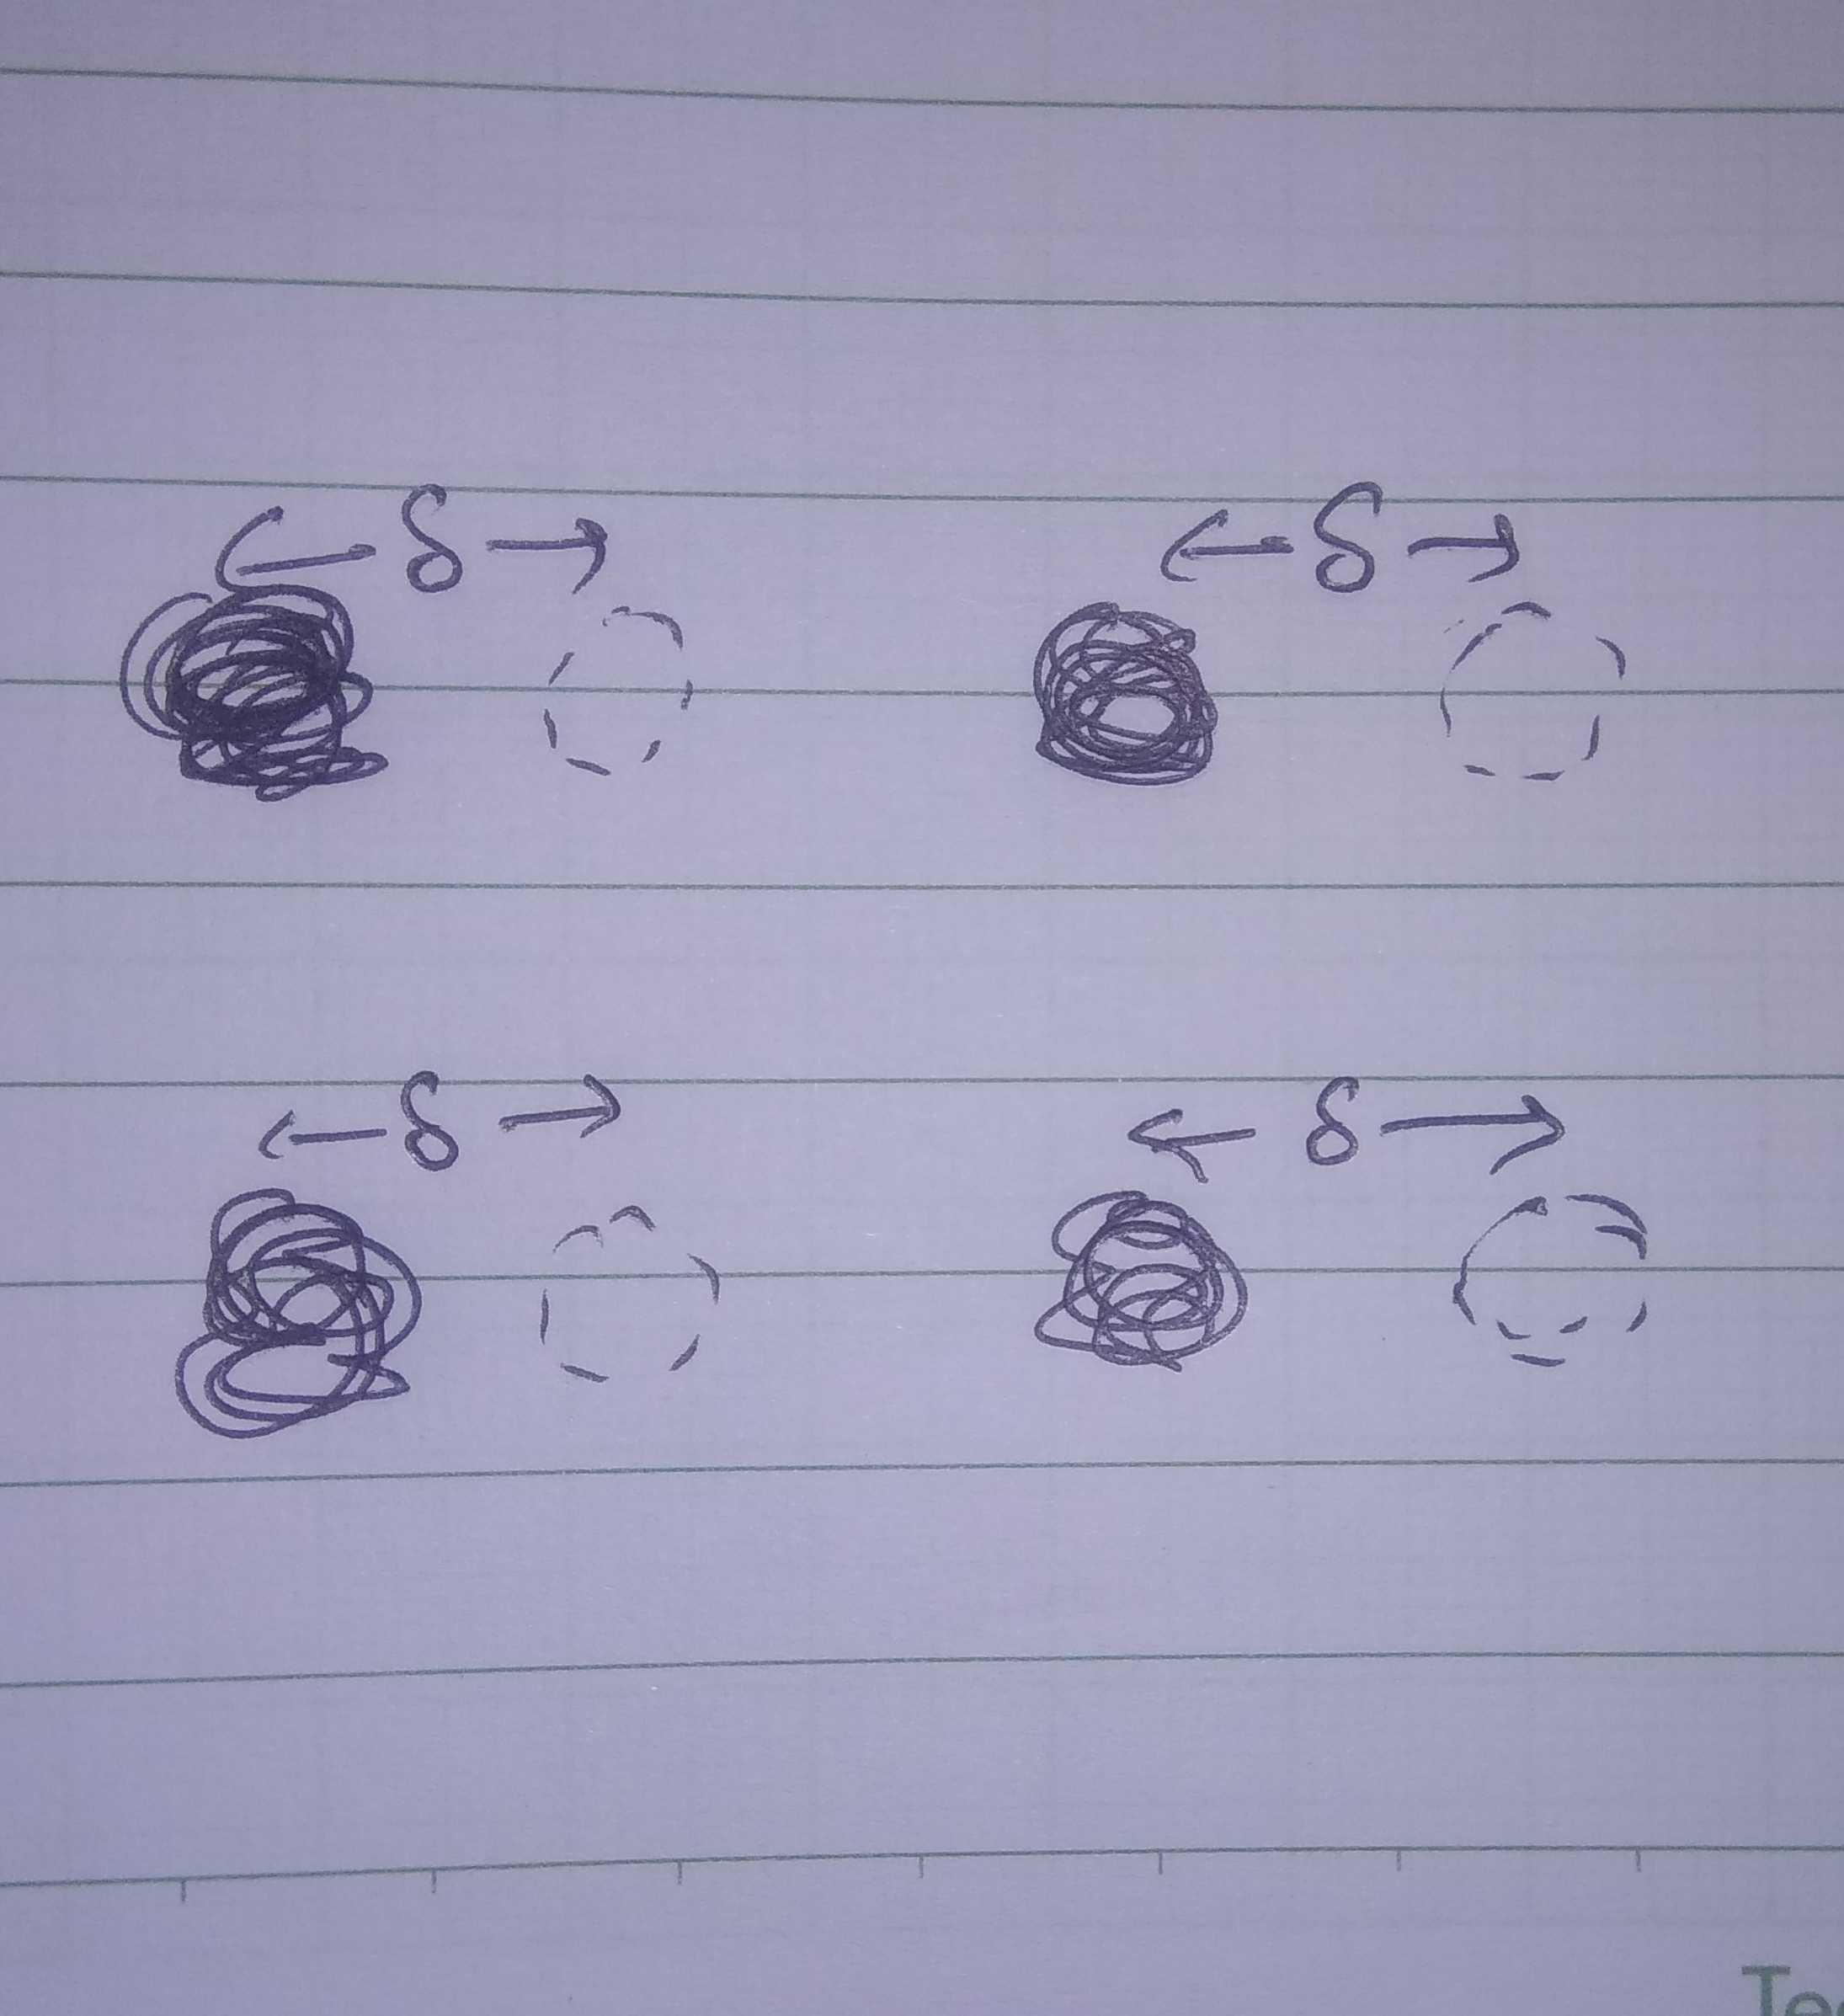
\includegraphics[scale=0.1]{IMG_20200722_230039.jpg}
\end{figure}

\begin{align*}
    \Delta P &\sim \frac{1}{\delta}\\
    \implies \Delta E &\sim \frac{1}{\mathcal{V}}*\frac{1}{\delta^2}\\
    \implies \Delta t &\sim \mathcal{V}\delta^2 \to\infty
\end{align*}

Hence ergodicity breaks and system only explores a reduced part of the phase-space.
\newpage

\subsection{What about non-zero $\vec{k}$ part of $H_{crystal}$ ?}
We collect terms with non-zero $\vec{k}$ part of the hamiltonian to get
\begin{equation}
    \sum_{\Vec{k}} \frac{1}{2m}\hat{P}(\Vec{k}) \hat{P}(\Vec{-k}) \;\mathcal{V} + \frac{m\omega^2}{2} \sum_{\vec{k}, \vec{\delta}} \hat{X}(\vec{k})\hat{X}(\vec{-k})\; 4sin^2(\frac{1}{2}\;\vec{k}\cdot\vec{\delta}) \mathcal{V}
\end{equation}
Let's work in 1-D for the time being. Then the $\vec{\delta}$ summation drops out to one term, 
\begin{equation*}
   \sum_{\vec{k}, \vec{\delta}} \hat{X}(\vec{k})\hat{X}(\vec{-k})\; 4sin^2(\frac{1}{2}\;\vec{k}\cdot\vec{\delta}) = \sum_{\vec{k}} \hat{X}^{\dagger}(\vec{k})\hat{X}(\vec{k})\; 4sin^2(\frac{1}{2}\;ka)
\end{equation*}
where a is the crystal spacing. So we arrive at
\begin{align}
    H_{int}\;&=\;\sum_{{k}} \displaystyle{\frac{1}{2m}}\hat{P}^{\dagger}(\Vec{k}) \hat{P}(\Vec{k}) \;\mathcal{V} + \frac{m\omega^2}{2} \sum_{\vec{k}} \hat{X}^{\dagger}(\vec{k})\hat{X}(\vec{k})\; 4sin^2(\frac{1}{2}\;ka)\mathcal{V}\\
    &= \sum_{{k}}\displaystyle{\frac{1}{2m}}\hat{P}^{\dagger}(\Vec{k}) \hat{P}(\Vec{k}) +  \frac{m\omega^2}{2} \hat{X}^{\dagger}(\vec{k})\hat{X}(\vec{k})\; 4sin^2(\frac{1}{2}\;ka)
\end{align}
which are a set of harmonic oscillators with frequencies $\omega_{k}\;=\;2\omega sin(\displaystyle{\frac{ka}{2}})$. \\
This corresponds to\textbf{ phonon-dispersion relation} for a 1d chain.\\
For small k, we get $\omega_k\;=\;(\omega a)k $, which corresponds to \textbf{goldstone modes}.\\
\newline
Elitzur's theorem - Local symmetries cannot be broken by such a mechanism.

\newpage
\subsection{Questions}

\begin{itemize}
    \item Can we smoothly go from one broken symmetry GS to another? What about to symmetric phase?
    \item Every time a global symmetry is broken, there $\exists$ a local variable that has long range order/correlations??
    \item SSB GS make a way to classify various phases of matter. And we know from day-day experience that one can typically change various parameters of the environment to trigger a phase transition. Then why is there a distinction between classical $\&$ quantum phase transitions?
\end{itemize}


\end{document}
